\documentclass{article}
\usepackage{arxiv}

\usepackage[utf8]{inputenc}
\usepackage[english, russian]{babel}
\usepackage[T1]{fontenc}
\usepackage{url}
\usepackage{booktabs}
\usepackage{amsfonts}
\usepackage{nicefrac}
\usepackage{microtype}
\usepackage{lipsum}
\usepackage{graphicx}
\usepackage{natbib}
\usepackage{doi}



\title{A template for the \emph{arxiv} style}

\author{  Полина Юрьевна Кривуля \\
	Факультет ВМК \\
    МГУ имени М.В.Ломоносова \\
	Москва, Россия \\
	\texttt{polina\_krivulya@mail.ru} \\
	%% examples of more authors
	\And
	Олег Валентинович Сенько \\
	Факультет ВМК \\
    МГУ имени М.В.Ломоносова \\
	Москва, Россия \\
	\texttt{senkoov@mail.ru}  \\
	%% \AND
	%% Coauthor \\
	%% Affiliation \\
	%% Address \\
	%% \texttt{email} \\
	%% \And
	%% Coauthor \\
	%% Affiliation \\
	%% Address \\
	%% \texttt{email} \\
	%% \And
	%% Coauthor \\
	%% Affiliation \\
	%% Address \\
	%% \texttt{email} \\
}
\date{}

\renewcommand{\shorttitle}{\textit{arXiv} Template}

%%% Add PDF metadata to help others organize their library
%%% Once the PDF is generated, you can check the metadata with
%%% $ pdfinfo template.pdf
\hypersetup{
pdftitle={A template for the arxiv style},
pdfsubject={q-bio.NC, q-bio.QM},
pdfauthor={David S.~Hippocampus, Elias D.~Striatum},
pdfkeywords={First keyword, Second keyword, More},
}

\begin{document}
\maketitle

\begin{abstract}
	В представленной работе осуществляется исследование задач, в которых целевая переменная определена через доверительные интервалы, а не посредством обучающей выборки. Основной целью данного исследования является изучение возможностей построения моделей для таких задач и проведение качественного анализа полученных результатов.

Одним из преимуществ данного способа определения целевой переменной является улучшение результатов по сравнению с моделями, использующими табличную обучающую выборку, благодаря возможности исключения выбросов. Также преимуществом данного подхода является его актуальность в случаях, когда наличие полноценной обучающей выборки невозможно.

В ходе исследования проводится математическое исследование различных методов построения моделей с использованием доверительных интервалов. Рассматриваются как классические статистические методы, так и алгоритмы машинного обучения. Данные методы применяются на эпидемиологических данных, проводится качественная оценка полученных результатов и сравнение их с моделями, обученными по классической табличной выборке.

Использование доверительных интервалов для определения целевой переменной способствует повышению надежности модели и уменьшению влияния случайных факторов на ее результаты. Данный подход особенно актуален в условиях, когда доступ к полноценным обучающим данным ограничен или невозможен.

\end{abstract}


\keywords{Машинное обучение \and Статистический анализ \and Эпидемиология \and Доверительные интервалы}

\section{Introduction}
Острые респираторные вирусные инфекции (ОРВИ) — наиболее распространенная патология, на долю которой приходится около 90\% всех инфекционных болезней. В Российской Федерации ежегодно болеют ОРВИ и гриппом более 30 млн человек, а суммарный экономический ущерб от респираторных вирусных инфекций оценивается в 40 млрд руб. в год. Большие экономические потери обусловлены вовлечением в эпидемический процесс трудоспособного населения, развитием осложнений, непродолжительным нестойким иммунитетом, определяющим повторные случаи заболевания. 

Вирусы, вызывающие респираторные инфекции, не являются эндемичными для какого-либо региона или страны и распространены повсеместно. Чаще эпидемии возникают в зимнее время, однако вспышки наблюдаются и в осенне-весенний период, а спорадические случаи ОРВИ — круглый год. Известно около 300 возбудителей респираторных инфекций, более 200 из них представители 4 семейств РНК-содержащих вирусов (ортомиксовирусы, парамиксовирусы, коронавирусы и пикорнавирусы) и 2 семейств ДНК-содержащих вирусов (аденовирусы и герпесвирусы).

 Цель данного исследования заключается в анализе и оценке характеристик нескольких типов вирусов, а именно гриппа, аденовируса, респираторно-синцитиального вируса (РС) и бокавируса. Для достижения данной цели проведен анализ набора симптомов, характерных для каждого из этих вирусов, а также учтены сезонные особенности. Ключевыми этапами данного исследования являются оценка статистической значимости симптомов и вычисление априорных и апостериорных вероятностей наличия каждого типа вируса. Для дальнейшего распознавания типа вируса по набору признаков использован алгоритм наивного байесовского классификатора. Результаты данного исследования могут быть полезны для лучшего понимания характеристик и распространения данных вирусов, а также для разработки эффективных методов профилактики и лечения.


\section{Headings: first level}
\label{sec:headings}

\lipsum[4] See Section \ref{sec:headings}.

\subsection{Headings: second level}
\lipsum[5]
\begin{equation}
	\xi _{ij}(t)=P(x_{t}=i,x_{t+1}=j|y,v,w;\theta)= {\frac {\alpha _{i}(t)a^{w_t}_{ij}\beta _{j}(t+1)b^{v_{t+1}}_{j}(y_{t+1})}{\sum _{i=1}^{N} \sum _{j=1}^{N} \alpha _{i}(t)a^{w_t}_{ij}\beta _{j}(t+1)b^{v_{t+1}}_{j}(y_{t+1})}}
\end{equation}

\subsubsection{Headings: third level}
\lipsum[6]

\paragraph{Paragraph}
\lipsum[7]



\section{Examples of citations, figures, tables, references}
\label{sec:others}

\subsection{Citations}
Citations use \verb+natbib+. The documentation may be found at
\begin{center}
	\url{http://mirrors.ctan.org/macros/latex/contrib/natbib/natnotes.pdf}
\end{center}

Here is an example usage of the two main commands (\verb+citet+ and \verb+citep+): Some people thought a thing \citep{kour2014real, hadash2018estimate} but other people thought something else \citep{kour2014fast}. Many people have speculated that if we knew exactly why \citet{kour2014fast} thought this\dots

\subsection{Figures}
\lipsum[10]
See Figure \ref{fig:fig1}. Here is how you add footnotes. \footnote{Sample of the first footnote.}
\lipsum[11]

\begin{figure}
	\centering
	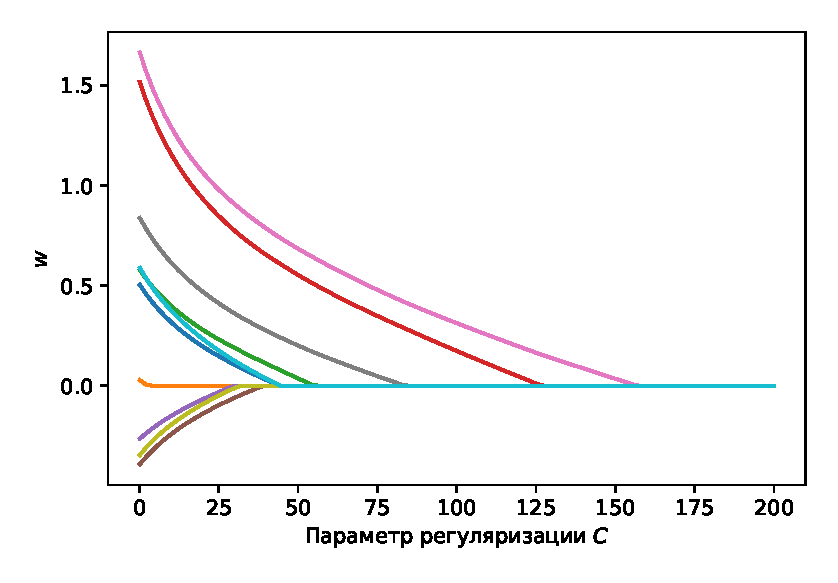
\includegraphics[width=0.5\textwidth]{../figures/log_reg_cs_exp.eps}
	\caption{Sample figure caption.}
	\label{fig:fig1}
\end{figure}

\subsection{Tables}
See awesome Table~\ref{tab:table}.

The documentation for \verb+booktabs+ (`Publication quality tables in LaTeX') is available from:
\begin{center}
	\url{https://www.ctan.org/pkg/booktabs}
\end{center}


\begin{table}
	\caption{Sample table title}
	\centering
	\begin{tabular}{lll}
		\toprule
		\multicolumn{2}{c}{Part}                   \\
		\cmidrule(r){1-2}
		Name     & Description     & Size ($\mu$m) \\
		\midrule
		Dendrite & Input terminal  & $\sim$100     \\
		Axon     & Output terminal & $\sim$10      \\
		Soma     & Cell body       & up to $10^6$  \\
		\bottomrule
	\end{tabular}
	\label{tab:table}
\end{table}

\subsection{Lists}
\begin{itemize}
	\item Lorem ipsum dolor sit amet
	\item consectetur adipiscing elit.
	\item Aliquam dignissim blandit est, in dictum tortor gravida eget. In ac rutrum magna.
\end{itemize}


\bibliographystyle{unsrtnat}
\bibliography{references}

\end{document}